\subsection{60}
\begin{myfrag}
Schreibe einen Ausdruck für die Einteilchen-Zustandssumme über die
quantisierten kinetischen Freiheitsgrade eines Gases. Was ist die
Hochtemperaturentwicklung der Energie und der spezifischen Wärme?
Welche Bedingung muss für die Längenskalen gelten, damit die
Hochtemperaturentwicklung gerechtfertigt ist?
\end{myfrag} \quad \\
$$ Z_1 = \sum \limits _r \exp ^{-\beta \epsilon_r}$$
Ebene Wellen mit Impuls $\vec{p} ,\left| \vec{p} \right\rangle \quad E_{\vec{p}} = \dfrac{p^2}{2m}$
Naive Erwartung: $$ Z_1 = \int d^3 p \exp ^{-\beta \dfrac{p^2}{2m} } $$
Problem: keine Orts, bzw. Volumenabhängigkeit. Endliches Volumen notwendig. \\[1ex]
Ein Teilchen im Potentialtopf hat quantisierte Impulse
$$ k_x = n x \dfrac{\pi}{L_x} \quad \vec{p} = \hbar(k_X,k_y,k_z) $$
$$ \Psi(x) \sim \sin (k_x x) \quad \sin (k_y y) \quad \sin (k_z z)$$
$$ Z_1 = \sum \limits _{n_x,n_y,n_z=1}^\infty \exp ^{ -\beta \dfrac{\hbar ^2 ( k_x^2 + k_y ^2 + k_z ^2)}{2m}} = Z_1^x Z_1^y Z_1^z$$
$$ Z_1 ^x = \sum \limits _{n_x = 1} ^\infty \exp ^{-\beta \dfrac{\hbar ^2 n x^2 \pi^2}{2m L_x^2}}$$
Randbedingungen dürfen am Ende keine Rolle spielen.
$$ Z_x = \dfrac{1}{2} \left( \sum \limits _{n_x = - \infty } ^\infty \exp ^ { - \alpha n_x ^2} -1 \right)$$
Was ist \qquad $\left( \sum \limits _{n_x = - \infty } ^\infty \exp ^ { - \alpha n_x ^2} -1 \right) = \sigma _3 (0, \exp ^{- \alpha } ) $ \\ elliptische Thetafunktion 3. Art (klassische Jacobi Thetafunktion)
$$ \alpha = \beta \dfrac{\pi ^2 \hbar ^2}{2m L_x ^2} = \dfrac{\pi}{4} \dfrac{\lambda ^2}{L_x^2}$$
Dualität 
$$\sum \limits _{n = - \infty } ^\infty \exp ^ { - \alpha n^2} = \sqrt{\dfrac{\pi}{\alpha} \sum \limits _{n = - \infty } ^\infty \exp ^ { - \pi ^2 \dfrac{n^2}{\alpha}}}$$
falls $\alpha << 1$ 
$$ \approx \sqrt{\dfrac{\pi}{\alpha }} \left( 1+ 2 \exp ^{ -\dfrac{\pi ^2}{\alpha } } + ...\right) $$
thermische Wellenlänge
$$ \lambda = \dfrac{h}{\sqrt{2 \pi m k_B T}} = \hbar \sqrt{\dfrac{2\pi}{m k_B T}} $$
offensichtlich $ \lambda << L_x$ für fast alle Fälle d.h. 
$$Z_x \approx \dfrac{1}{2} \sqrt{\dfrac{\pi}{\alpha}} = \dfrac{1}{2} \sqrt{\dfrac{\pi 4 L_x^2}{\pi \lambda ^2}} = \dfrac{L_x}{\lambda }$$
$$ \Rightarrow Z_1 = Z_1^x Z_1^y Z_1^z = \dfrac{V}{\lambda ^3} $$ 
mit " richtiger Normierung", aber ansonsten $Z_1 \propto V(k_B T ) ^\frac{3}{2} $ wie im klassischen Fall \\
Anmerkung: gilt auch für periodische Randbedingung \\[1.5ex]
$ E = \dfrac{\partial ln Z_1}{\partial \beta} = \dfrac{3}{2} k_B T \\[1.5ex]
C_V = \dfrac{3}{2} k_B$
\subsection{61}
\begin{myfrag}
Was ist das Verhalten der spezifischen Wärme für die Vibrationsfreiheitsgrade
eines Molekülgases?
\end{myfrag} \quad \\
Weitere Freiheitsgrade im realen Gas \\
Schwingungsmoden = Normalmoden \\
Jede Mode entspricht einem Quantenoszillator
$$ Z_{vib} = \sum \limits _{n=0} ^\infty \exp ^{ -\beta \hbar \omega n} = \dfrac{1}{1-\exp ^{-\beta \hbar \omega}}$$
$$ E_{vib}= - \dfrac{\partial lnZ}{\partial \beta} = \dfrac{\hbar \omega}{\exp ^{\beta \hbar \omega }-1}$$
$$ C_V = \dfrac{\partial E}{\partial T} = k_B \left( \dfrac{\hbar \omega }{k_B T} \right) \dfrac{\exp ^{\hbar \omega \beta }}{\exp ^{\hbar \beta \omega } -1}$$
\subsection{62}
\begin{myfrag}
Was ist die Zustandssumme über die quantisierten Rotationsfreiheitsgrade
eines Moleküls aus zwei verschiedenen Atomen? Berechne die
Tieftemperatur-Entwicklungen der Zustandssumme, der Energie und der
spezifischen Wärme.
\end{myfrag} \quad \\
$$ E_{rot} = \dfrac{\hbar ^2 l(l+1)}{2I}$$
\glqq zusätzliche\grqq Energie, näherungsweise für alle Schwingungsmoden. \\
Summation über alle möglichen Drehimpulsquantenzahlen:
$$ Z_{rot} = \sum \limits _{l=0}^\infty (2l+1) \exp ^{-\beta E_{rot} } = \sum \limits _{l=0} ^\infty (2l+1) \exp ^{-l(l+1)\dfrac{\theta _{rot}}{T}} \qquad \qquad \theta _{rot} = \dfrac{\hbar ^2}{2Ik_B} $$
Führt zu Entartung in z-Richtung $-l \leqslant m \leqslant l$ \\[1.5ex]
Tieftemperaturentwicklung: Reihentwicklung
$$ Z_{rot} \approx 1 + 3 \exp ^{- \dfrac{2 \theta _{rot}}{T}}+5 \exp ^{\dfrac{6 \theta _{rot}}{T}}$$
$$ ln(1+\epsilon) \approx \epsilon -\dfrac{\epsilon^2}{2}$$
$$ln(Z_{rot} \approx 3 \exp ^{\dfrac{-2 \theta _{rot}}{T}} - \dfrac{9}{2} \exp ^{\dfrac{-4 \theta _{rot}}{T}} + \sigma \left( \exp ^{\dfrac{-2 \theta _{rot}}{T}} \right)$$
$$\left\langle E_{rot} \right\rangle = - \dfrac{\partial lnZ_{rot}}{\partial \beta} \approx 6k_B \theta_{rot} \exp ^{\dfrac{-2 \theta _{rot}}{T}} - 18k_B \theta_{rot}\exp ^{\dfrac{-4 \theta _{rot}}{T}} + ...$$
$$C_V = \dfrac{\partial E}{\partial T} = 12 k_B \left( \dfrac{\theta_{rot}}{T}\right) ^2 \exp ^{\dfrac{-2 \theta _{rot}}{T}} - 72k_B \left( \dfrac{\theta_{rot}}{T}\right) ^2 \exp ^{\dfrac{-4 \theta _{rot}}{T}} + ...$$
\begin{figure}
\begin{center}
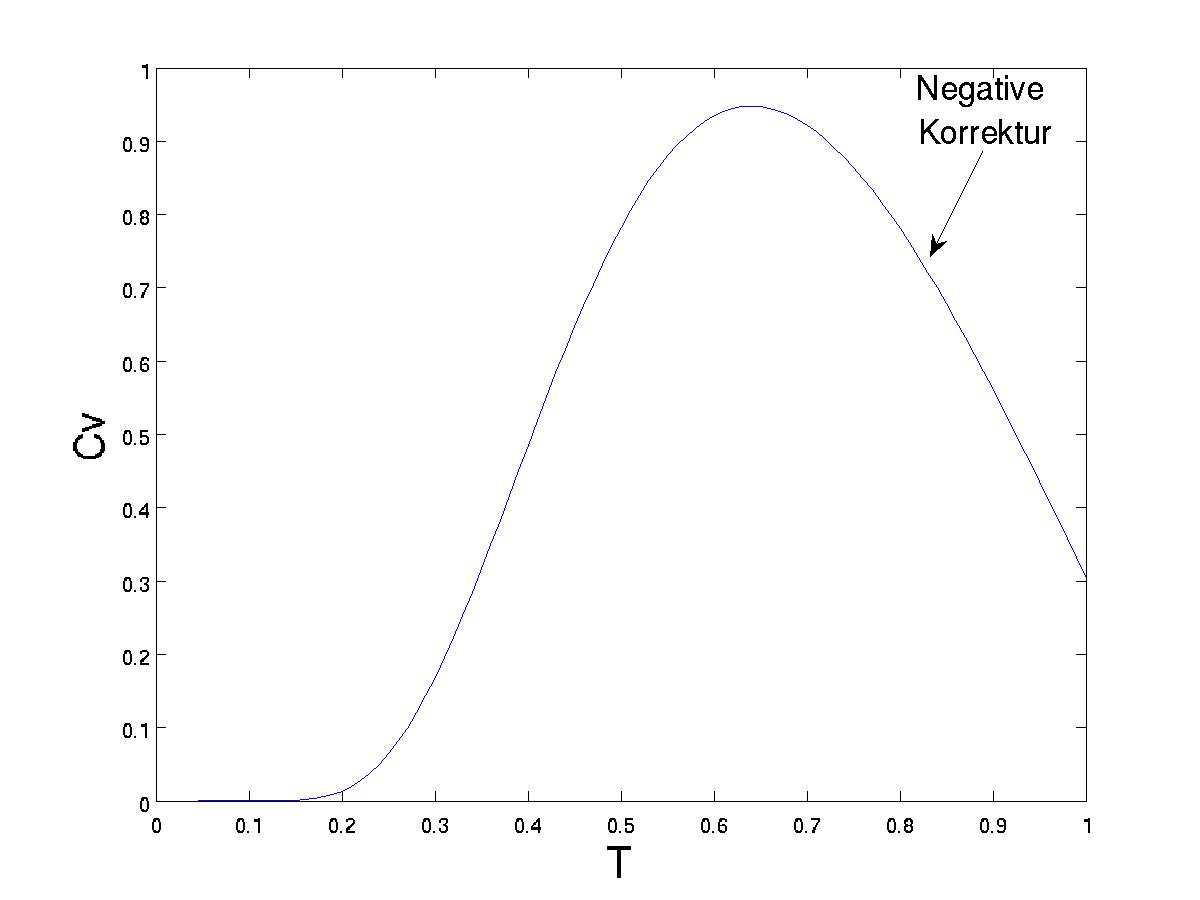
\includegraphics[width= 10cm]{Bilder/Frage62.jpg} 
\caption{$C_V-T$ Diagramm mit negativ Korrektur (= 2 klassische Rotationsfreiheitsgrade (Senkrecht zur Molekühl Achse)) }
\end{center}
\end{figure}
\subsection{63}
\begin{myfrag}
Erkläre wie eine Hochtemperatur-Entwicklung der Rotationszustandssumme
gemacht werden kann (die MacLaurin Summen Formel sei gegeben). Erkläre,
warum cv(T) ein Maximum als Funktion der Temperatur durchläuft.
\end{myfrag} \quad \\
Hochtemperaturentwicklung: Integralnäherung \\[2ex]
Euler-Maclarin Integralnäherung \\[1ex]
Allgemein: $$ \sum \limits _{l=0}^\infty f(l) \approx \int _0 ^\infty f(l) \dif l + \dfrac{f(0)}{2} - \dfrac{f'(0)}{12}+\dfrac{1}{710} f''(0)+ ...$$
 $$ f(l) = ( 2l+1) \exp ^{-l(l+1)\dfrac{\theta _{rot}}{T}}$$
 $$ \int _0^\infty \dif l (2l+1)\exp ^{-l(l+1)\dfrac{\theta _{rot}}{T}} = \int _0 ^\infty \dif x \exp ^{-x\dfrac{\theta _{rot}}{T}} = \dfrac{T}{\theta_{rot}} \qquad mit \quad x = l(l+1) \quad \dif x = (2l+1) \dif l$$
 $\dfrac{f(0)}{2}=\dfrac{1}{2}$ \\[1.5ex]
 
 $\dfrac{f'(l)}{12}= \dfrac{1}{12} ( 2 \exp ^{-l(l+1)\dfrac{\theta _{rot}}{T}} + (2l+1) \exp ^{-l(l+1)\dfrac{\theta _{rot}}{T}}\left( -2l\dfrac{\theta_{rot}}{T}-\dfrac{\theta_{rot}}{T} \right)$ \\[1.5ex]
 $\dfrac{f'(0)}{12} = \dfrac{1}{12} \left( 2 - \dfrac{\theta_{rot}}{T} \right)$
 $$\Rightarrow Z_{rot} \approx \dfrac{T}{\theta_{rot}} + \dfrac{1}{2} - \dfrac{1}{12}\left(2-\dfrac{\theta_{rot}}{T} \right) \approx \dfrac{T}{\theta_{rot}} + \dfrac{1}{3} + \dfrac{\theta_{rot}}{12T} = \dfrac{T}{\theta_{rot}} \left( 1+ \dfrac{\theta_{rot}}{3T} + \dfrac{1}{12}\left(\dfrac{\theta_{rot}}{T} \right) ^2 + ... \right)$$
$$ ln Z _{rot} \approx ln \dfrac{T}{E_{rot}} + \dfrac{\theta_{rot}}{3T} + \dfrac{1}{90} \left( \dfrac{\theta _{rot}}{T}\right)^2 + ...$$
$$ E_{rot} = - \dfrac{\partial lnZ_{rot}}{\partial \beta } \approx k_B T - \dfrac{k_B \theta_{rot}}{3} - \dfrac{1}{45} \dfrac{k_B \theta_{rot}^2}{T}+...$$
$$ C_V = \dfrac{\partial E_{rot}}{\partial T} \approx k_B + \dfrac{1}{45} \dfrac{k_B \theta_{rot}^2}{T}+...$$
\begin{figure}[H]
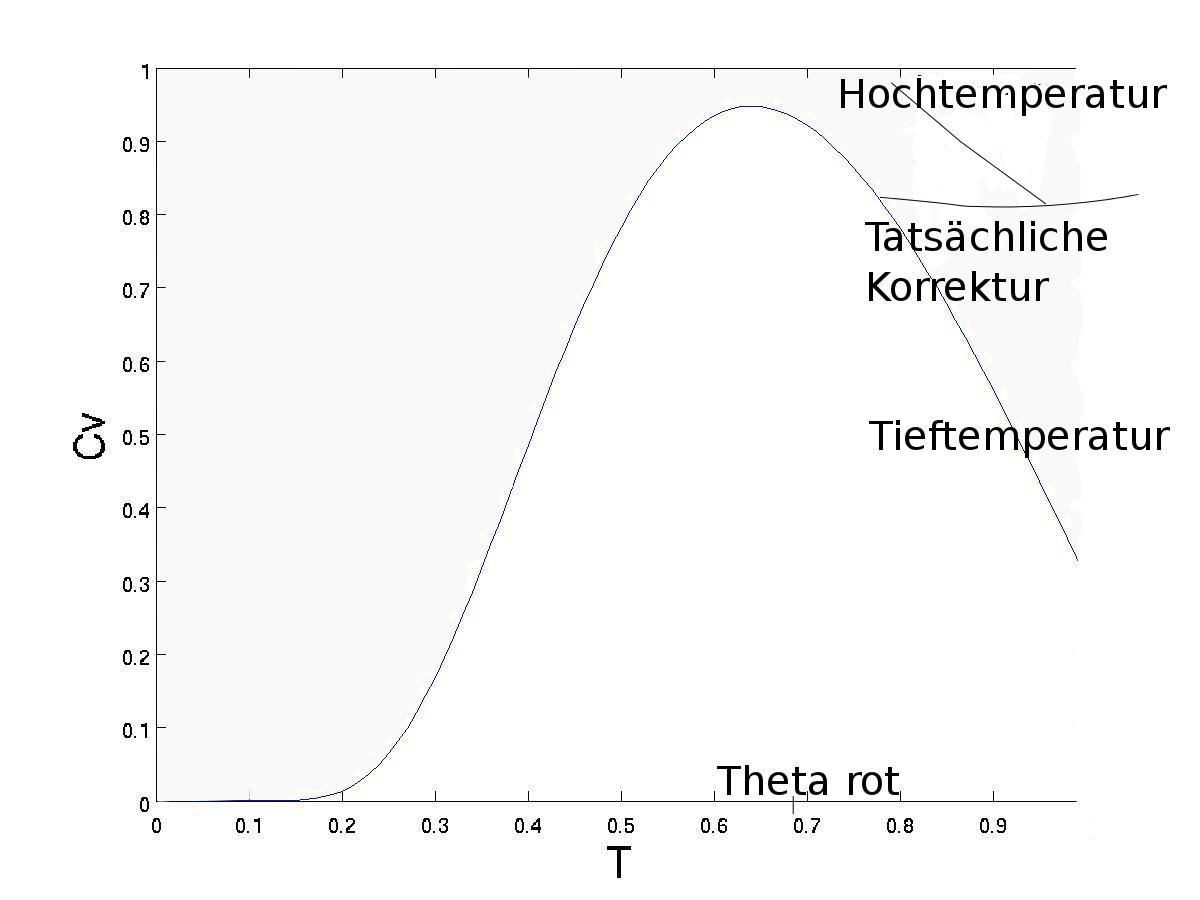
\includegraphics[width= 10cm]{Bilder/Frage63.jpg} 
\caption{$C_V -T $ Diagramm mit den Unterschiedlichen Korrekturen. Besitzt Maximum da lücke voll besetzt, danach wieder runter bis wieder aufgefüllt ist.}

\end{figure}
\subsection{64}
\begin{myfrag}
Erkläre allgemein wie sich die Eigenschaften eines diskreten Spektrums
(Entartung, Energieabstände) im Temperaturverlauf von cv(T) widerspiegeln
(mit Beispiel).
\end{myfrag}
\subsection{65}
\begin{myfrag}
Was muss bei der Zustandssumme über die quantisierten
Rotationsfreiheitsgrade eines zwei-atomigen Moleküls beachtet werden, wenn
das Molkül aus identischen Atomen besteht? Wie sieht dann die
Zustandssumme für die Fälle aus, dass der Kernspin s ganz- oder halbzahlig
ist?
\end{myfrag} \quad \\
Bei Molekühlen mit ununterscheidbaren Atomen muss Quantenstatistik berücksichtigt werden. \\
Inteferenz mit Periode $\pi $ und nicht nur mit $ 2 \pi $ \\[1.5ex]
Grundsätzlich bei ununterscheidbaren Teilchen 
\\
\begin{itemize}
\item Symmetrische Wellenfunktion $ \Psi (\vec{r} _1 , \vec{r}_2 , \sigma _1 , \sigma _2 ) = \Psi (\vec{r} _2 , \vec{r}_1 , \sigma _1 , \sigma _2 ) $ für Bosonen
\item antisymmetrische Wellenfunktion $\Psi (\vec{r} _1 , \vec{r}_2 , \sigma _1 , \sigma _2 ) = - \Psi (\vec{r} _2 , \vec{r}_1 , \sigma _2 , \sigma _1 )$ für Fermionen
\item $\sigma $ \glqq interne \grqq Quantenzahl z.B Spin (Bosonen Ganzzahlig Fermionen Halbzahlig
\end{itemize}
Oftmals Annahme: \\[1.5ex] 
Ort unt interne Friheitsgrade sind nicht verschränkt.
d.h. $$\Psi (\vec{r} _1 , \vec{r}_2 , \sigma _1 , \sigma _2 ) = \phi (\vec{r} _1 , \vec{r}_2) \chi ( \sigma _1 , \sigma _2 )$$
$$ \phi _\pm (\vec{r} _1 , \vec{r}_2) = \pm \phi (\vec{r} _2 , \vec{r}_1)$$
$$\chi_\pm ( \sigma _1 , \sigma _2 ) = \pm \chi ( \sigma _2 , \sigma _1 )$$
Für Bosonen $$ \Psi_B = \phi_+ \chi_+ \quad oder \quad \Psi_B = \phi_-\chi_- $$
Für Fermionen: $$ \Psi_\pm = \phi_- \chi_+ \quad oder \quad \Psi_\pm = \phi_+\chi_-$$
Drehimpuls: Wellenfunktion muss gerade unter $ \vec{r} \rightarrow - \vec{r} $ sein (Relativkoordinate)\\
d.h. $\phi_+ = \Psi_{nl}(r) Y_{lm}(\theta, m)$ sind gerade, für l teilbar durch 2 \\[1.5ex]
$\phi_- $ für ungerade l l=1,3,5... \\[2ex]
Wasserstoff $H_2$ \\[1.5ex]
Fermionen mit $S=\dfrac{1}{2}$ \\[1.5ex]
$\left| \chi_+ \right\rangle = \left. \begin{array}{c} 
\left| \uparrow \uparrow \right\rangle \\
\left| \downarrow \downarrow \right\rangle \\
\frac{1}{\sqrt{2}} (\left| \downarrow \uparrow \right\rangle + \left| \uparrow \downarrow \right\rangle )

\end{array} \right\rbrace $ triplets (symmetrisch) \\
$\left| \chi_- \right\rangle = \left. \begin{array}{c} \frac{1}{\sqrt{2}} (\left| \downarrow \uparrow \right\rangle + \left| \uparrow \downarrow \right\rangle ) \end{array} \right\rbrace $ \\[1.5ex]
Für allgemeinen Spin S \\
$(2s+1)(2s+1) \quad $ Zustände gesamt \\[1.5ex]
$s(2s+1) \quad$ ungerade unter Vertauschung\\[1.5ex]
$(s+1)(s+1) \quad $ gerade unter Vertauschung \\[2ex]
$$Z_{H_2} = \sum \limits _{alle Zust"ande} \exp ^{-\beta \epsilon } = \sum \limits _{l\ ungerade} \sum \limits _ {triplet} \exp^{-\beta \frac{l(l+1)\hbar^2}{2I}}(2l+1) + \sum \limits _{l\ gerade} \sum \limits _ {singulett} \exp^{-\beta \frac{l(l+1)\hbar^2}{2I}}(2l+1)$$ $$ = 3 Z_{ungerade} + Z_{gerade}$$
Allgemein Boson mit $ s= 0,1,2,...$ 
$$ Z_{rot} = (s+1)(2s+1) Z_{gerade} + s(2s+1) Z_{ungerade} $$ Wobei $Z_{gerade}$ die Anzahl der Spinwellenfunktionen \\[1.5ex]
Gesamtzahl Spinzustände $(2s+1)^2$ \\[1.5ex]
Fermionen: $\dfrac{1}{2},\dfrac{3}{2},\dfrac{5}{2}, ...$
$$Z_{rot} = 2(s+1)Z_{gerade} + (s+1)(2s+1) Z_{ungerade} $$ 
\subsection{66}
\begin{myfrag}
Was versteht man unter Ortho- und Para-Wasserstoff? Wie kann das
Verhältnis von Ortho und Para-Wasserstoff im Gleichgewicht berechnet
werden? Gegen welche Werte strebt das Verhältnis für sehr große und für
sehr kleine Temperaturen?
\end{myfrag} \quad \\
Singulett: Para-Wasserstoff mit $\phi (\vec{r} _1 , \vec{r}_2) = \phi (\vec{r} _2 , \vec{r}_1)$ symmetrisch , $Z_{gerade}$ \\[1.5ex]
Triplett: Ortho-Wasserstoff mit $ \phi (\vec{r} _1 , \vec{r}_2) = - \phi (\vec{r} _2 , \vec{r}_1) $ antisymmetrisch ,$Z_{ungerade}$ 
$$ \Psi_{para} = \Psi ^S (\vec{r} _1 , \vec{r}_2) \otimes \chi (S=0) $$ 
$$ \Psi_{ortho} = \Psi ^a (\vec{r} _1 , \vec{r}_2) \otimes \chi (S=1,m_s) $$
$H_2$:
$$ Z_{rot} = 3 Z_{ungerade} + Z_{gerade} $$
$$ T=0 \rightarrow Grundzustand \qquad \dfrac{Z_{ungerade}}{Z_{gerade}} \rightarrow ^{T \rightarrow 0} 0 \qquad d.h. 100 \% \ Para \quad 0 \% \ ortho $$
Allgemein: \\[1.5ex]
Parawasserstoff: 
$$ \dfrac{Z_{gerade}}{3Z_{ungerade} + Z_{gerade}} \rightarrow \left\lbrace \begin{array}{c c} 1 & T \rightarrow 0 \\
\frac{1}{4} & T \rightarrow \infty
\end{array} \right. $$
für $T \rightarrow \infty : Z_{ungerade} = Z_{gerade} \propto \frac{T}{\theta_{rot}}$
\subsection{67}
\begin{myfrag}
Erkläre die Darstellung von fermionischen und bosonischen Wellenfunktionen
mit Hilfe von Besetzungszahlen. Was versteht man unter
statistischer Abstoßung bzw. Anziehung?
\end{myfrag}\quad \\
Interferrenzeffekte \glqq automatisch \grqq in der Symmetrie (Bosonen) bzw. Antisymmertrisch (Fermionen) unter Vertauschung enthalten.
$$ \begin{array}{l} \left\lbrace \left| r \right\rangle \right\rbrace = \left\lbrace \left| a \right\rangle , \left| b \right\rangle, \left| c \right\rangle \right\rbrace$$\\[2ex]
$$ \left| a \right\rangle _1 \otimes \left| a \right\rangle _2 \qquad \left| a \right\rangle _1 \otimes \left| b \right\rangle _2 \qquad \left| a \right\rangle _1 \otimes \left| c \right\rangle _2 \\
\left| b \right\rangle _1 \otimes \left| a \right\rangle _2 \qquad ... \\
...
\\
\qquad \qquad \qquad \qquad \qquad \qquad \quad \ \left| c \right\rangle _1 \otimes \left| c \right\rangle _2

\end{array} $$
Symmetrische Wellenfunktionen
$\Rightarrow$ 6 Bosonische Zustände (Basisizustände) \\
TODO
\subsection{68}
\begin{myfrag}
Mache eine vereinfachte Herleitung für die Bose-Einstein und die Fermi-
Dirac Verteilungen als Summe über Besetzungszahlen eines Zustandes für
den Fall dass es kein chemisches Potential gibt.
\end{myfrag}
\subsection{69}
\begin{myfrag}
Beschreibe das Konzept des Großkanonischen Ensembles. Definiere die
großkanonische Zustandssumme, das großkanonische Potential $\Phi$, die
Fugazität z und das chemische Potential $\mu$.
\end{myfrag}